\section{Proposed Research}
% Including method or approach and expected difficulties
% This must constitute about 50\% of the text of the written proposal: 7-8 pages
% Clear statement of the work to be undertaken and must include:
% Objectives for the period of the proposed work and expected significance
% Relation to the present state of knowledge in the field and to work in progress at Michigan/elsewhere
% Expected research program sequence
% Decision points expected during the course of the research
% Methods of data reduction, evaluation, interpretation and presentation

% https://en.wikipedia.org/wiki/Folding_funnel#/media/File:Folding_funnel_schematic.svg
%\begin{figure*}[t]
%\begin{center}
%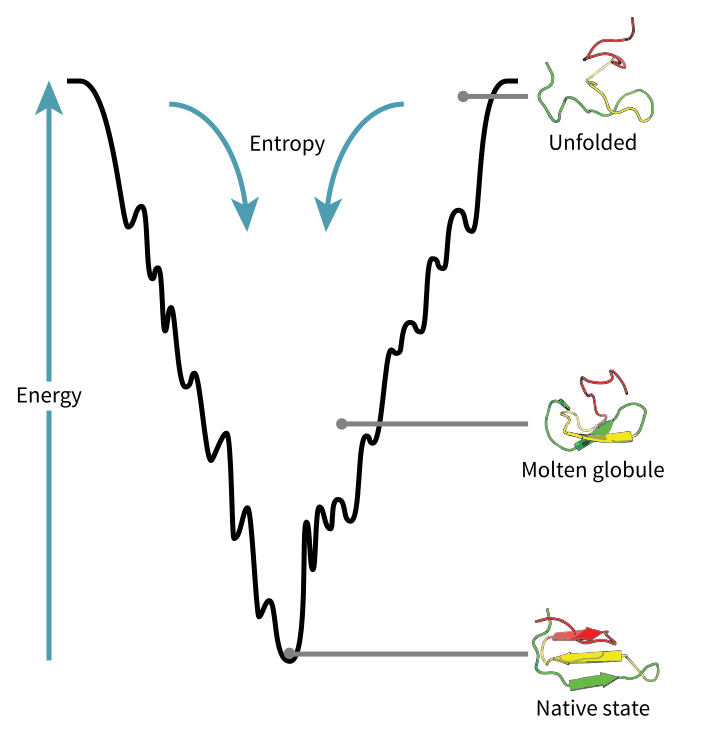
\includegraphics[width=3in]{../figures/foldingfunnel.png}
%\caption{The diagram sketches how proteins fold into their native structures by minimizing their free energy. (Source: Wikipedia}
%\label{fig:funnel}
%\end{center}
%\end{figure*}


% =====
% IMPORTANCE
% =====

\subsection*{Question to be addressed}

While much research energy has been focused on understanding how simple interactions can lead to complex structures or how addressable structures can be programmed for self assembly, there is a middle ground with relatively sparse literature.
How can we \textit{optimize} the amount of self-assembly instruction given to a system to successfully assemble a target structure?

To assemble Archimedean tilings from regular polygons, Millan \textit{et al.} incrementally applied attractive patches to particles until the target structure was assembled \cite{Millan_2014_ACSNano}.
Their heuristics of increasing interaction specificity mirror the increasing specificity detailed above: hard interactions only, then symmetric patches, shape-specific patches, and edge-specific patches.
The authors were able to demonstrate that a decision tree with just three nodes was sufficient to determine the level of instruction needed to reach a given target structure.

%While work on quantifying the amount of information in a specific bond can help differentiate what type of interaction is more specific, 

Instead of focusing on minimum instructions, work on protein folding has focused on identifying key intermediate states formed during the folding process \cite{Jacobs_2016_BiophysicalJournal}.
Jacobs \textit{et al.} demonstrated that indeed, there are preferred transition states along pathways that lead to successful folding.
In such systems, while the final structure is fully defined by the primary structure of the protein, sampling all possible configurations to find the final state would take an impossibly long time (this is known as ``Levinthal's paradox,'' and will be further discussed later in the proposal).
The folding of a protein introduces geometric considerations in which local native bonds preferentially form to scaffold the folding \cite{Dill_1993_PNAS}.

Thus, while proteins and patchy colloidal assembly appear to be very disparate approaches to this topic, combined they suggest an intriguing idea. 
Could a minimally sufficient set of non-specific interactions be combined with a constrained geometry (in the form of folding) to allow for self-assembly of a target structure?  

%In this work, I propose developing such a heuristic, using a simple assembly system composed of nets of 3 of the Platonic solids.
%I then will use this heuristic to improve assembly yield on poor-assembling systems.
%Disconnectivity trees will be used to explore the free energy landscape of folding in these systems, offering an alternative view for determining why some bonds are more critical to assembly than others.
%Finally, I will use this ability to identify the minimal set of critical bonds needed for assembly to embed pluripotent behavior in a folded sheet.
%I expect this to be a colloidal analog of the folding sheet with actuators studied by Desmaine, Rus, and colleagues \cite{An_2011_Robotica}. 


% =====
% MODEL
% =====

\subsection*{Proposed model}

I propose studying this question using nets of the five Platonic solids as described in \cite{Dodd_2018_unpublished}.
These nets can be implemented as rigid bodies connected by harmonic springs, with non-specific attractive patches on the edges of each net ``face.''
Molecular dynamics (implemented in HOOMD-blue \cite{HOOMD_2008, HOOMD_2015}) will be used to simulate assembly.

In a forth-coming study from the Glotzer lab using this system \cite{Dodd_2018_unpublished}, the authors find that for the same target shape, compact nets with more leaves assemble most reliably (in agreement with \cite{Azam_2009_PlosOne}).
By investigating the assembly behavior for shapes with fewer possible net constructions (i.e. tetrahedon, cube, and octahedron), they are then able to use these features to predict which nets will assemble for shapes with a wide variety of possible net constructions (i.e. dodecahedron and icosahedron). 
Additionally, they observe that reliable assembly is due to the formation of local native (that is, present in the final structure) bonds early in the simulation which in turn bring non-local contacts together to be folded next (i.e. cooperatively) \cite{Dill_1993_PNAS}.
They posit that as each net folds, it freezes out the fewest possible number of degrees of freedom, thereby maximizing the conformational entropy along the folding pathways.

This finding closely mirrors what is already known in studies of protein folding.
In 1968, Cyrus Levinthal posed the following thought experiment, come to be known as ``Levinthal's Paradox'' \cite{Levinthal_1969}.
Proteins are known to fold on the order of a second-- however, if proteins explored all their possible degrees of freedom they would never be able to assemble.
A polypeptide with 100 residues would have 99 peptide bonds, and therefore 198 different phi and psi bond angles.
If each of those bond angles could be in one of three stable conformations, the protein would potentially have to sample $3^{198}$ different conformations to reach its native configuration.
Randomly sampling such a large number of configurations in search of the native configuration is not even possible in the life-time of the universe-- and thus, Levinthal's Paradox.

\begin{wrapfigure}{r}{0.5\textwidth}
  \begin{center}
    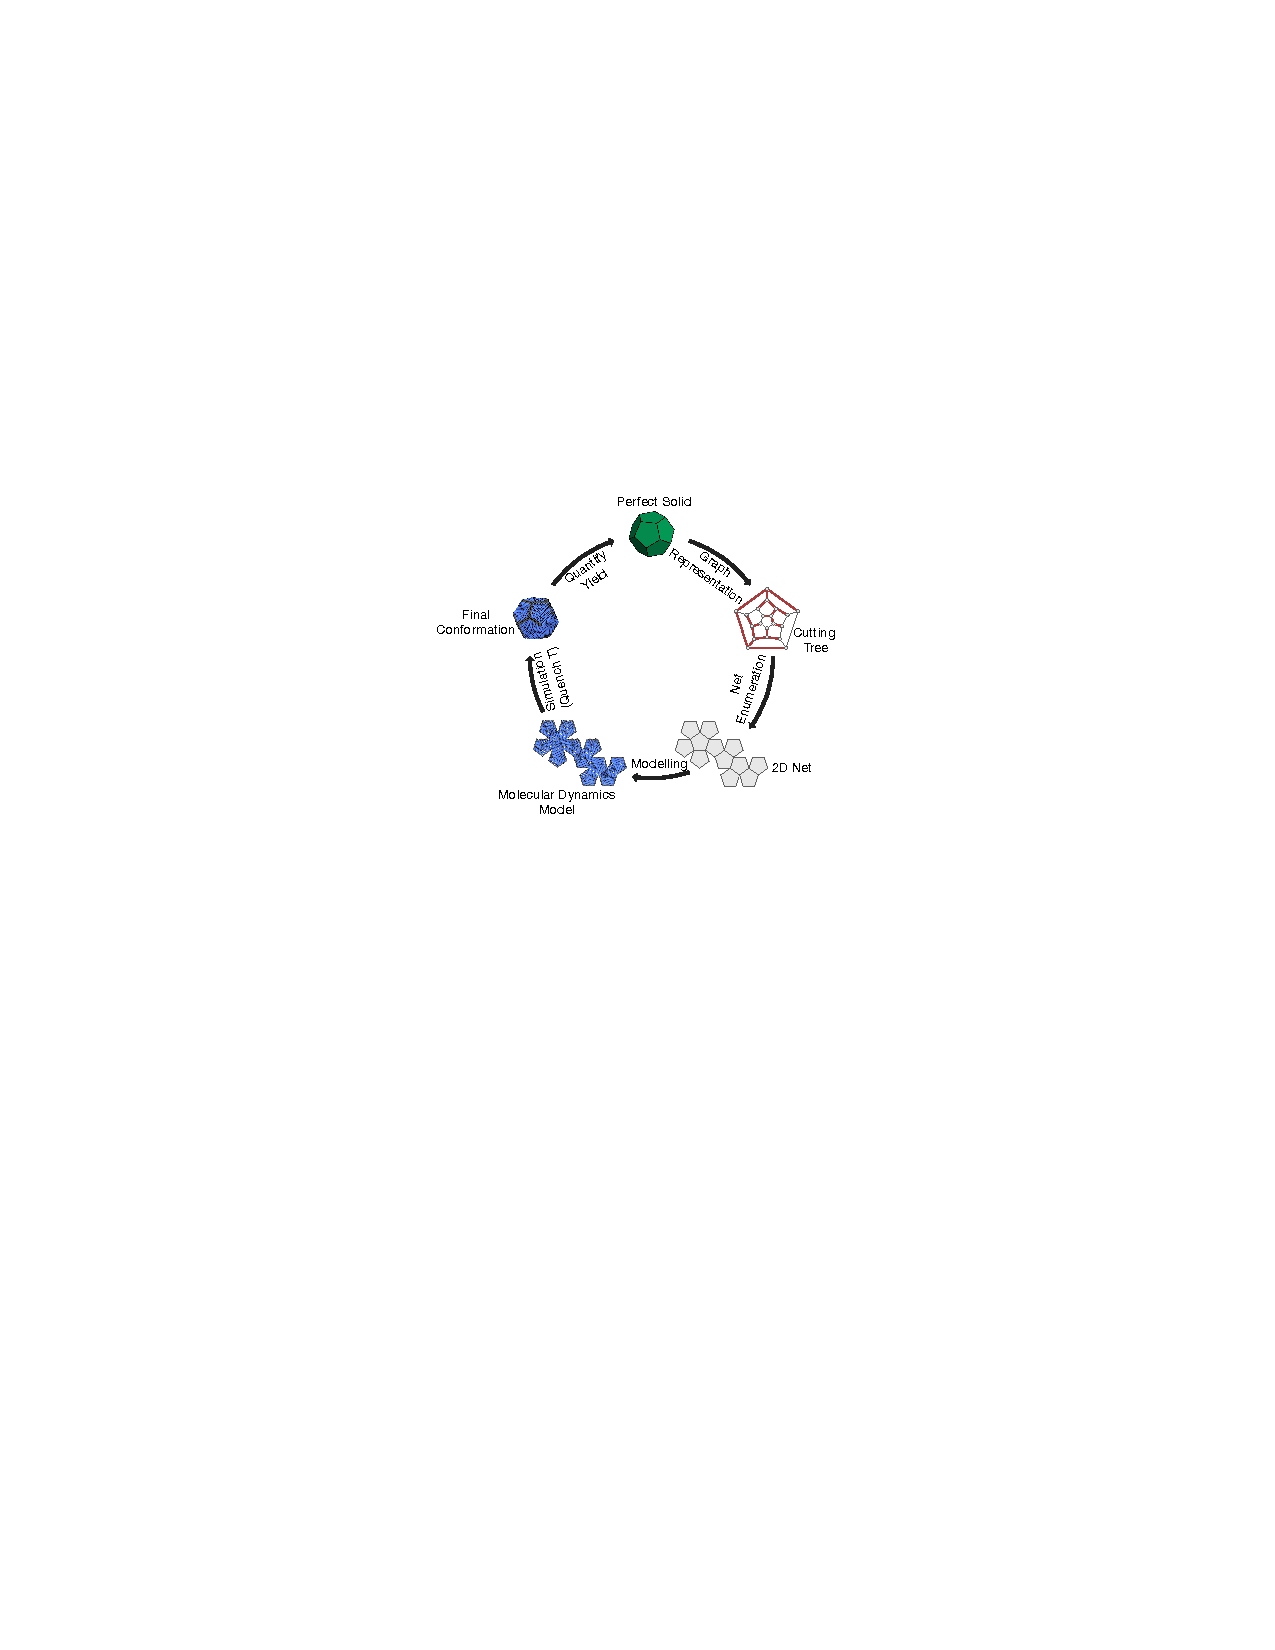
\includegraphics[width=0.48\textwidth]{../figures/nets.pdf}
  \end{center}
  \caption{
  \textbf{Model, proposed work}:
  Process for developing nets from Platonic solids, from \cite{Dodd_2018_unpublished}}
\end{wrapfigure}

Levinthal posited that biological folding times could be explained by the formation of local, native contacts which would stabilize the structure.
Indeed, over 20 years later, these small biases (on the order of just a few $kT$) towards the native configuration were mathematically demonstrated to result in biologically realistic protein folding times \cite{Zwanzig_1992_PNAS,Martinez_2014_JChemEd}.
In analyses of real-world folding times, protein folding speeds correlate with the topology of the native protein.
Fast folders usually have mostly local structure, such as helices and tight turns, whereas slow folders usually have more non-local structure, such as $\beta$-pleated sheets \cite{Plaxco_1998_JMolBio}.
Further work on elucidating experimental protein kinetics detected the partially folded intermediates transition states in the folding process posited by Levinthal \cite{Dill_2007_CurrOpinStructBio}. 

%Statistical mechanical models of protein folding uncovered that assembly does not follow single microscopic pathway.
%Instead, protein folding is characterized by funnel-shaped energy landscapes, with entropy increasing as proteins assemble with decreasing free energy as shown in Figure \ref{fig:funnel} \cite{Dill_1997_Nature}.

Given that we are able to replicate complex findings from protein folding in this simple system of a folding net, this suggests that we can continue to use this system as a toy model for developing theory of tailored self-assembly.
In proteins, Levinthal posited that some local contacts may act as ``nucleation points in the folding process''.
Though the interactions of the edges in the folding nets are not specific like those in proteins, the same critical local contacts are observed in the folding process.

This suggests that the combination of geometry and attraction serve to make some local bonds in folding nets more effective than others.
In turn, it may be possible to identify bonds that are more critical to assembly than others. 
If we are able to rank the importance of edge bonds on the yield of an assembly pathway, then it stands to reason that we can determine which interactions are the minimally sufficient set needed to guide assembly into a target structure. 

% =====
% PROJECT ONE: CRITICAL BONDS, WHAT DO YOU NEED TO ADD TO GET ASSEMBLY?
% =====
\begin{figure}[tb]
\begin{center}
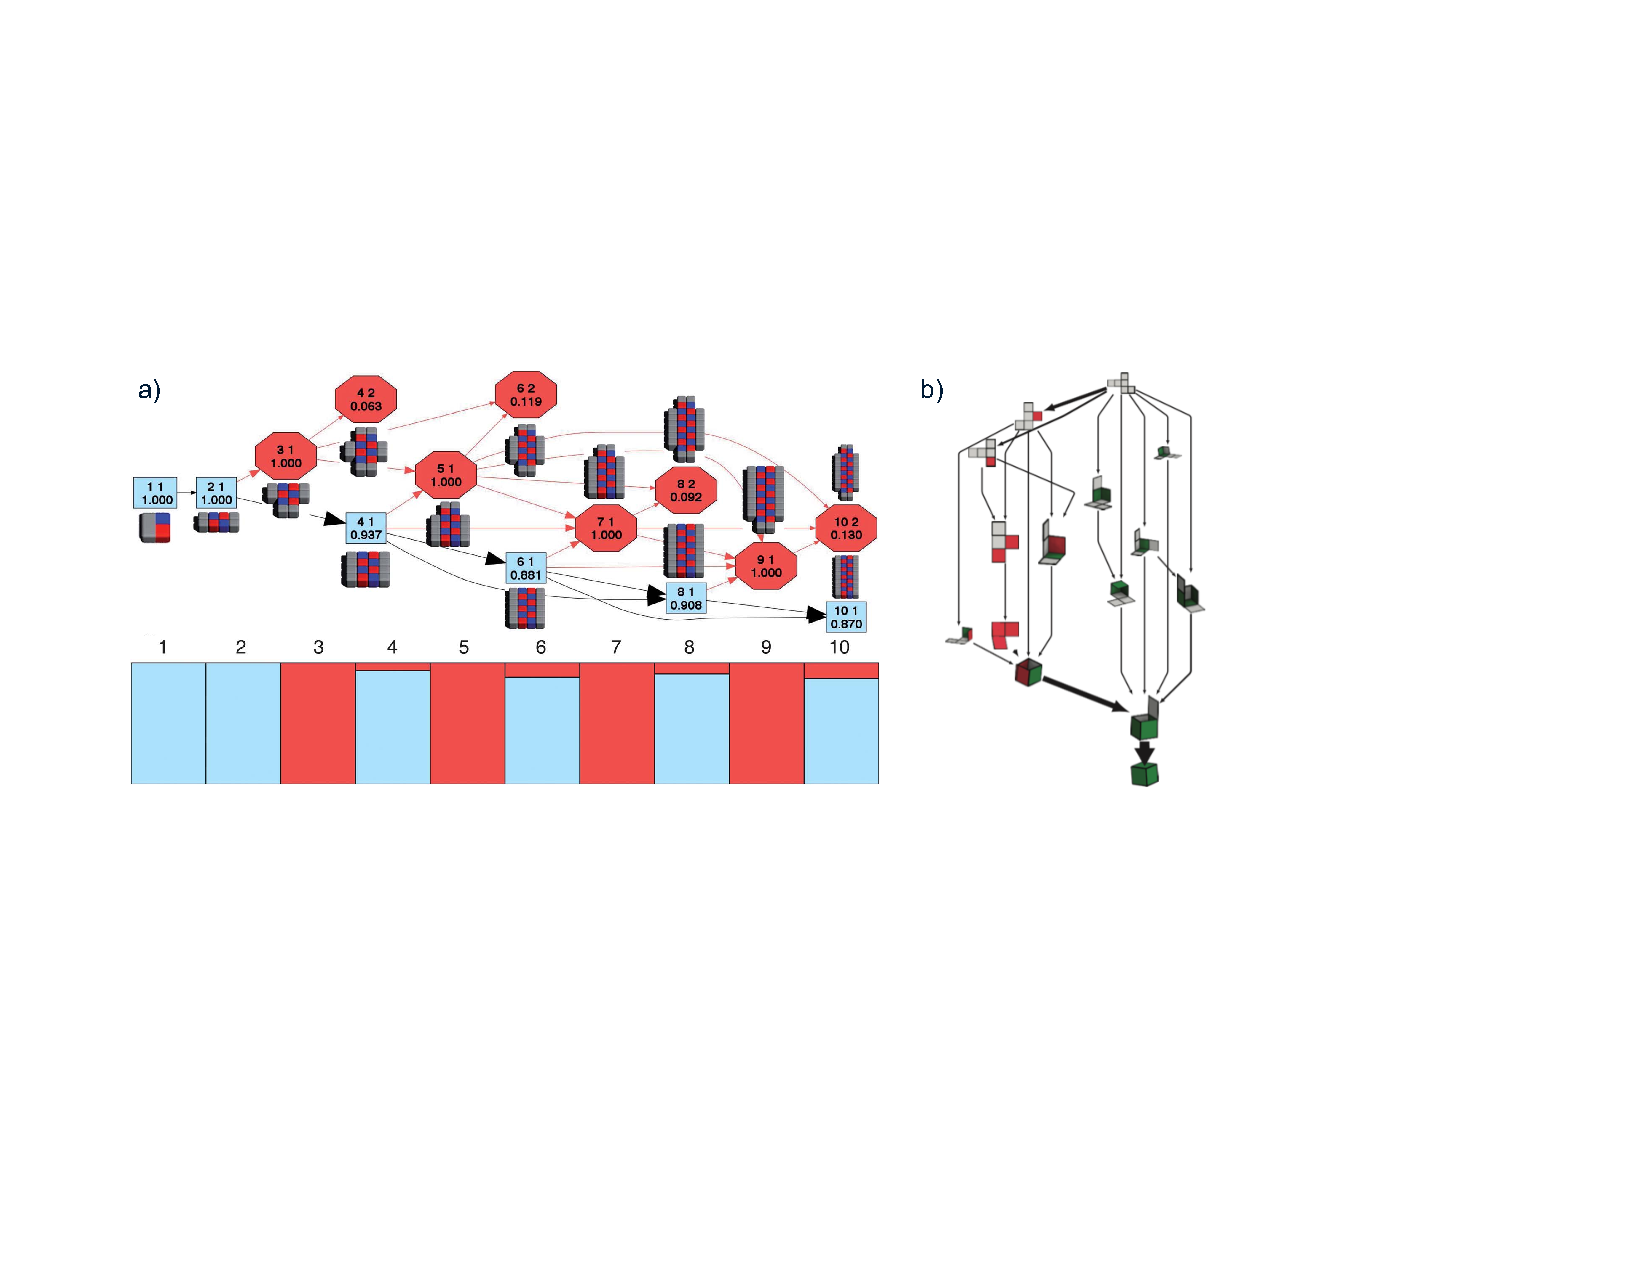
\includegraphics[width=6.5in]{../figures/bubba.pdf}
\caption{
\textbf{Transition state analysis}:
(a) Analysis of assembly pathways and relative populations of building blocks into target assembly patterns. \cite{Jankowski_2012_SoftMatter}.
Labels at each node indicate the size of a cluster, its energy level for its size (1 for lowest, 2 for second-lowest, etc.), and its probability compared to clusters of the same size. 
(b) Significant transition states and folding fluxes for net of a cube \cite{Dodd_2018_unpublished}. 
}
\label{fig:bubba}
\end{center}
\end{figure}

\subsection*{Project 1: Define measure of pathway information}

\textit{Background}

Previously, work by Jankowski \textit{et al.} measure the flux through and relative energies of transition states en route to a target pattern formation \cite{Jankowski_2012_SoftMatter}. 
In that study, they sought to enable pathway design by identifying key transition ``cluster'' building blocks that a system would need to go through for the pathway to end in successful assembly. 
Here, we propose using this same approach but instead to identify key bonds that must form en route to a successfully-folded net (see Figure \ref{fig:bubba}).

Next, we need an approach to quantifying how correlated a given bond is with successful assembly.
Huntley \textit{et al.} have developed an analogous information-theory-driven approach for the specificity of lock and key bonds, which we can adapt for our uses \cite{Huntley_2016_PNAS}. 

For a system of $N$ distinct locks ($x_1,x_2,...,x_N\in X$) with unique partner keys ($y_1,y_2,..., y_N \in Y$), we can calculate that binding between a lock $x_i$ and key $y_j$ will occur with probability $p(x_i,y_j)=e^{-{\beta}E_{ij}}/Z$, where $Z$ is a normalization factor such that $\sum_{i,j}p(x_i,y_j)=1$ and $E_{ij}$ is the binding energy.

In information theory, the mutual information quantifies how predictive the message received is of the signal that sent it.
In the case of lock and key bonds, we can think about having a mutual information that is a measure of how predictive the identity of a lock $x_i$ is of the identity of a key $y_j$ bound to it.
Specifically, we can write the mutual information $I(X;Y)$ as:
\begin{equation}
I(X;Y) = \sum_{x_i{\in}X,y_j{\in}Y} p(x_i,y_j)\log_2\frac{p(x_i,y_j)}{p(x_i)p(y_j)}
\end{equation}
where $p(x_i)$ is the marginal distribution of $x_i$, representing the total probability of seeing $x_i$ in a bound pair [and similarly $p(y_j)$].

In the folding nets, instead of the state being a lock bonded with a key, we are instead measuring whether the presence of a bond is correlated to the net proceeding to folding (i.e. measuring the yield).
That is, if bond $x_i$ exists at a transition state, how predictive is this of the transition state proceeding to a successful folded final state?

\textit{Proposed work}

First, our goal will be to define a metric that measures the likelihood of a bond being a part of a successful assembly pathway.
The first approach to this will be taking pathways already enumerated in \cite{Dodd_2018_unpublished} and calculating their eventual yield in assembling the target structure, as done in \cite{Jankowski_2012_SoftMatter}.
With this correlation in hand, we can then calculate a first-pass mutual information measure between the existence of a bond in the structure and the assembled structure of the net.

This will provide an approximation of the ranking importance of the bonds formed in the assembly of a net.
In case this approach is an over-simplification, we will need to find a way to account for cooperativity between bonds in the folding process.
For example, one bond ($x_1$) on its own may be a poor predictor that the structure will assemble, but when present with another bond $x_2$ becomes highly predictive of successful assembly into the target structure.
One key advantage of the nets system is that its possible configurations are countable.
Thus, we could incrementally seed nets with combinations of edge bonds and measure their yield to fully characterize cooperativity between bonds in the folding pathway.

With this metric in hand, we can test whether ``seeding'' a poor-folding net with a critical bond will improve the folding yield.
We will take a poor-folding net, seed it with a bonded edge we have estimated to be most critical to successful folding, and then allow system to proceed with folding.
If our metric is good, we expect that we will be able to improve the yield through these bond additions.
By incrementally adding critical bonds until a net folds, we will also be able to measure the minimum sufficient instruction needed for a given net to assemble at a given yield.

From this ratio of instruction (input) to measured yield (output), we can imagine calculating a type of ``instruction efficiency''.
Poor folding nets that require multiple bonds to be seeded to fold to a target structure would be said to be of low efficiency, while nets that folded the target structure with perfect yield even with no seeded bonds would be of high efficiency.

Ideally, we will be able to use these findings to predict which bonds will be critical in assembling a net we have not already characterized.
Can we predict which bonds are going to be the most critical from heuristics we can develop based on mutual information between bonds and assembled structures in studied nets?


% =====
% PROJECT TWO: DISCONNECTIVITY GRAPHS
% =====

\subsection*{Project 2: Develop energy landscapes for identifying kinetic barriers to assembly}

\textit{Background}:

Seeding a structure with a critical bond, like those identified in Project 1, can help the assembly process avoid searching a local energetic minimum en route to the global minimum.
In Project 1, we take a transition state flux-based probabilistic view to identify which bonds correlate with high yields.
However, we also need to understand the underlying energetics to understand the mechanisms by which these bonds work.
We would expect that critical bonds are those that prevent a configuration from exploring particularly deep (and thus energetically costly) local minima.

Disconnectivity graphs convert an energy landscape into a network of energy minima and transition states \cite{Smeeton_2014_JCompChem,Becker_1997_JChemPhys,Wales_2017_JChemPhys,Wales_2006_JChemPhysB}.
This network reflects the connectivity between local energy basins.
From disconnectivity graphs, we would expect to be able to identify large kinetic traps in the folding of these nets, and identify the location of transition states with bonds relative to those kinetic traps.
Configurations that are likely to assemble reliably have few side-branches which have higher free energies than the target structure.
Poor assembling configurations, on the other hand, have wide disconnectivity graphs, or deep local minima basins that are separated by an early transition state from the global minimum.
Example disconnectivity graphs are shown in Figure \ref{fig:disconnectivity}.


\begin{figure}[bt]
\begin{center}
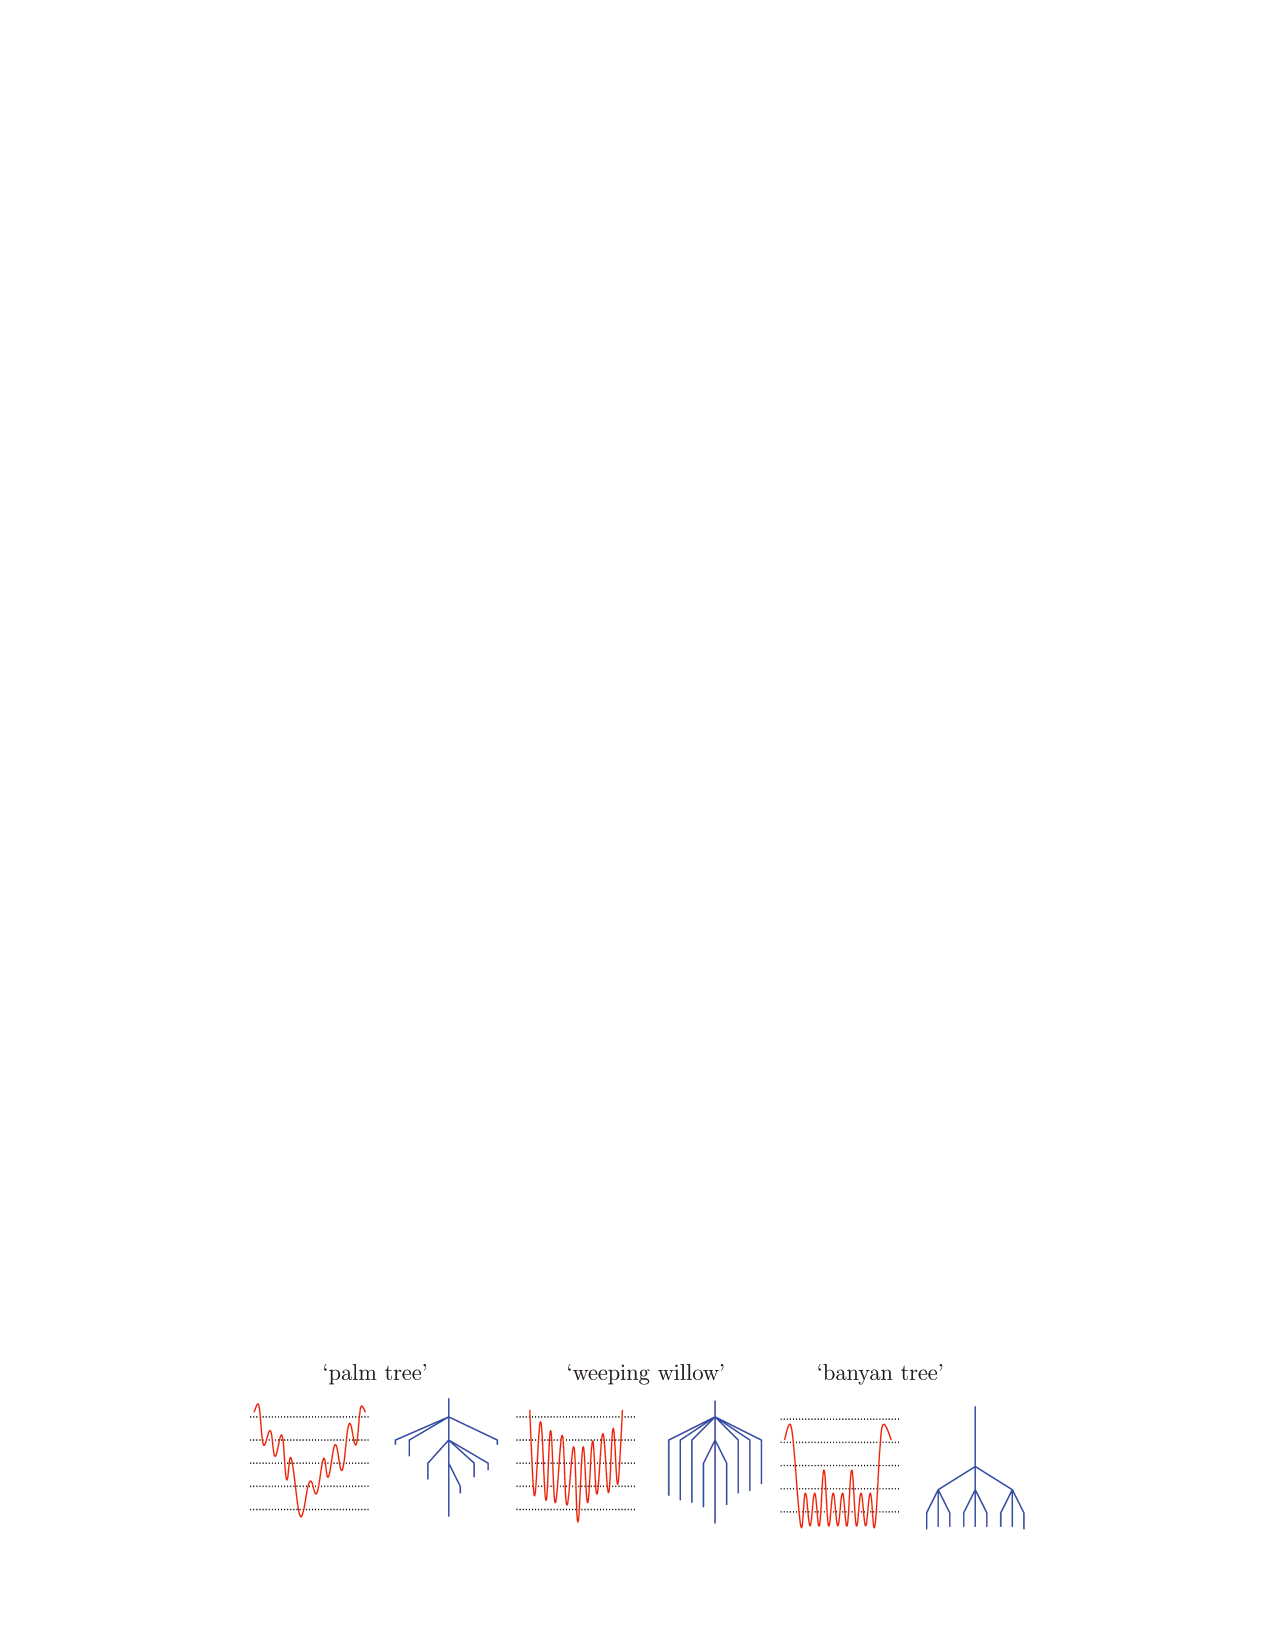
\includegraphics{../Figures/disconnectivity.pdf}
\caption{
\textbf{Disconnectivity graphs}:
One-dimensional potential energy functions (left) and the corresponding disconnectivity graphs (right) for representative energy landscapes \cite{Wales_2006_JChemPhysB}.
The dotted lines indicate the energies at which analysis was performed to find local minima.
Proteins are often characterized by the ``palm tree'' configuration and funneled energy landscape.
For a net with a ``willow tree'' characteristic disconnectivity graph, we might expect that a seeding bond which is able to start the folding at the second major split from the top would lead to an increased folding yield.}
\label{fig:disconnectivity}
\end{center}
\end{figure}


\textit{Proposed work}:

First, we will develop disconnectivity graphs for this family of nets.
David Wales' group at the University of Cambridge has developed a code base that can be used to develop disconnectivity graphs, though applying it to new systems is non-trivial.
A PhD graduate of Wales' who was previously a post-doc in the Glotzer lab has agreed to assist with adapting this method to a folding system.
With disconnectivity graphs in hand, we will then look to understand what they can tell us about (i) nets that fold well organically and (ii) the role of critical bonds in navigating assembly kinetics.
Can we identify features of nets that correlate with ``palm tree'' style connective graphs, versus less assembly-friendly disconnectivity graph topologies?

First, we might expect that nets that fold well without assistance correspond to a narrower energetic funnel, like those seen in protein foldings.
Identifying characteristics of nets that correspond with narrower energetic funnels would be a novel view of self-assembly in folding systems.

Second, we hypothesized that critical bonds would help the assembly avoid kinetic traps.
We would expect these to be bonds that move the transition state from a node with multiple branches leading to locally deep minima, down to a node closer to the global minimum.
We can also work in reverse.
Given a disconnectivity graph, we can follow the transition states up the tree from the global minimum to find the most energetically favorable pathway from the starting net.
As with nets with narrow energetic funnels, studying such pathways may give us further energetic insight into why some nets fold better than others.

While this proposed work seems straightforward, a variant this project has previously been attempted with a Glotzer lab member visiting the Wales group to develop disconnectivity graphs for our assembly work.
The student found the code base to be fairly inflexible and difficult to apply to our systems.
In this student's judgement, it would almost be easier to re-write the disconnectivity graph generating code for our systems than adapt the version that exists for this folding problem.

Getting the analysis code working will be a non-trivial aspect of this work.
However, having this tool on hand could have broad-reaching uses within our group for characterizing assembly pathways, which is an area of increasing interest among Glotzer lab PhD students.


% =====
% PROJECT THREE: PLURIPOTENT MATERIALS
% =====

\subsection*{Project 3: Design pluripotent nets from minimal instructions}

\textit{Background}

Traditionally, the goal of self-assembly is to form one targeted structure from constituent components.
However, systems which would self-assemble into different structures under different assembly conditions could be of use in applications ranging from sensing to colloidal robotics.
Such systems would be ``pluripotent'', as they contain the instructions to form multiple different stable assemblies from the same starting materials.

Currently, the closest precursors to \textit{colloidal} pluripotent materials are systems whose configuration changes when subjected to external fields.
In one example, Han \textit{et al.} developed hinged chains of electromagnetic blocks, whose hinges could be manipulated using a magnetic field to ``fold'' into different conformations, analogously to different secondary structures forming from an amino acid primary structure \cite{Han_2017_SciAdv}.

However, folding architectures have been widely explored as a \textit{macroscopic} means of using a pluripotent starting material (often a sheet with seeded creases for folding) and accessing a variety of structures.

In studies of origami folding algorithms, Desmaine and colleagues developed a fold-finding algorithm to move between multiple folded configurations of a 4-box pleated sheet, while minimizing the number of actuators (folds), groups, or edges \cite{An_2011_Robotica}.
Trolley \textit{et al.} demonstrate that such heat-senstitive seams could be used to make macro-scale self-folding origami that could be triggered by uniform heating, rather than targeted stimulus of the folds \cite{Tolley_2014_SMS}.
And in an impactful paper from early 2017, a robust example of algorithmically-designed 3D reconfigurable materials based on space-filling tessellations demonstrated the ability to move from one structure to another without undergoing an intermediate ``unfolding'' step \cite{Overvelde_2017_Nature}. 

In Projects 1 \& 2, we will have rigorously characterized methods of folding in a colloidal system.
Here in Project 3, we will seek to apply these methods to creating colloidal-scale pluripotent materials.


\textit{Proposed work}

We will start with a pluripotent folding precursor.
The simplest system, based on Projects 1 \& 2, would be to take nets of the Platonic solids and have two target states: one of the folded state, and the other a local minimum made the preferred state through the folding design process.
For example, the lowest free energy configuration for some octahedra nets is actually an open boat-like structure which has higher rotational entropy than the assembled octahedron \cite{Dodd_2018_unpublished}. 

Unlike in the previous projects, we cannot use non-specific bonds throughout the structure and ``seed'' bonds along critical edges prior to letting assembly proceed. 
Instead, we will ``seed'' using specific attractive patches along the critical edges for one of the target structures.
When we want to begin folding towards a target structure, we will ``turn on'' the attractive patches to drive those critical bonds to form.

Our previous work developing the information capacity of net/bond combinations will allow us to define the minimum set of bonds we will need to specify to fold each target state.
In doing so, in specifying bonds for the first structure, we should ideally have un-specified bonds that can be used to form the second.
Of course, it is possible that given the geometry of the nets, some edges will need to be seeded in both the target structures.
For the sake of this theoretical demonstration, we can have three types of specific patches on the edges: (1) specific only with those patches needed in configuration 1, (2) specific only in configuration 2, and (3) specific in both.

For simplicity, assembly would transition between pluripotent states through the unfolded state.
Depending on the success of elucidating kinetic barriers and transition states in Project 2, an additional challenge for this Project could be designing pathways that avoided unfolding completely, or expanding to more complex starting materials like the 4-box pleated sheet studied by \cite{An_2011_Robotica}. 

Turning bonds ``on/off'' would experimentally still rely upon assembly conditions, though we can imagine this change in attraction happening in response to some change in solvent conditions (e.g. a sensing response).
Developing a variant of the system that could be synthesized in lab would be a significant step forward in programmable colloidal self-assembly.
Working with collaborators to test this model in the lab would very likely extend the reach of the theories developed here.
(Note that this is not proposed as part of the thesis work, but would be a stretch-goal.)



